% !TEX root = PREN2_Dokumentation.tex
\section{Methoden}
\subsection{\gls{SoDa}}
Das Projektmanagement wird mit dem hybriden Projektvorgehen \gls{SoDa} der Hochschule Luzern durchgeführt. 
SoDa wurde dabei bereits schon in vorhergehenden Softwareentwicklungsmodulen eingesetzt und hat sich hier bewährt. Die Userstories werden dabei auch im \gls{GitLab} erfasst.  
\begin{figure}[H]
	\centering
	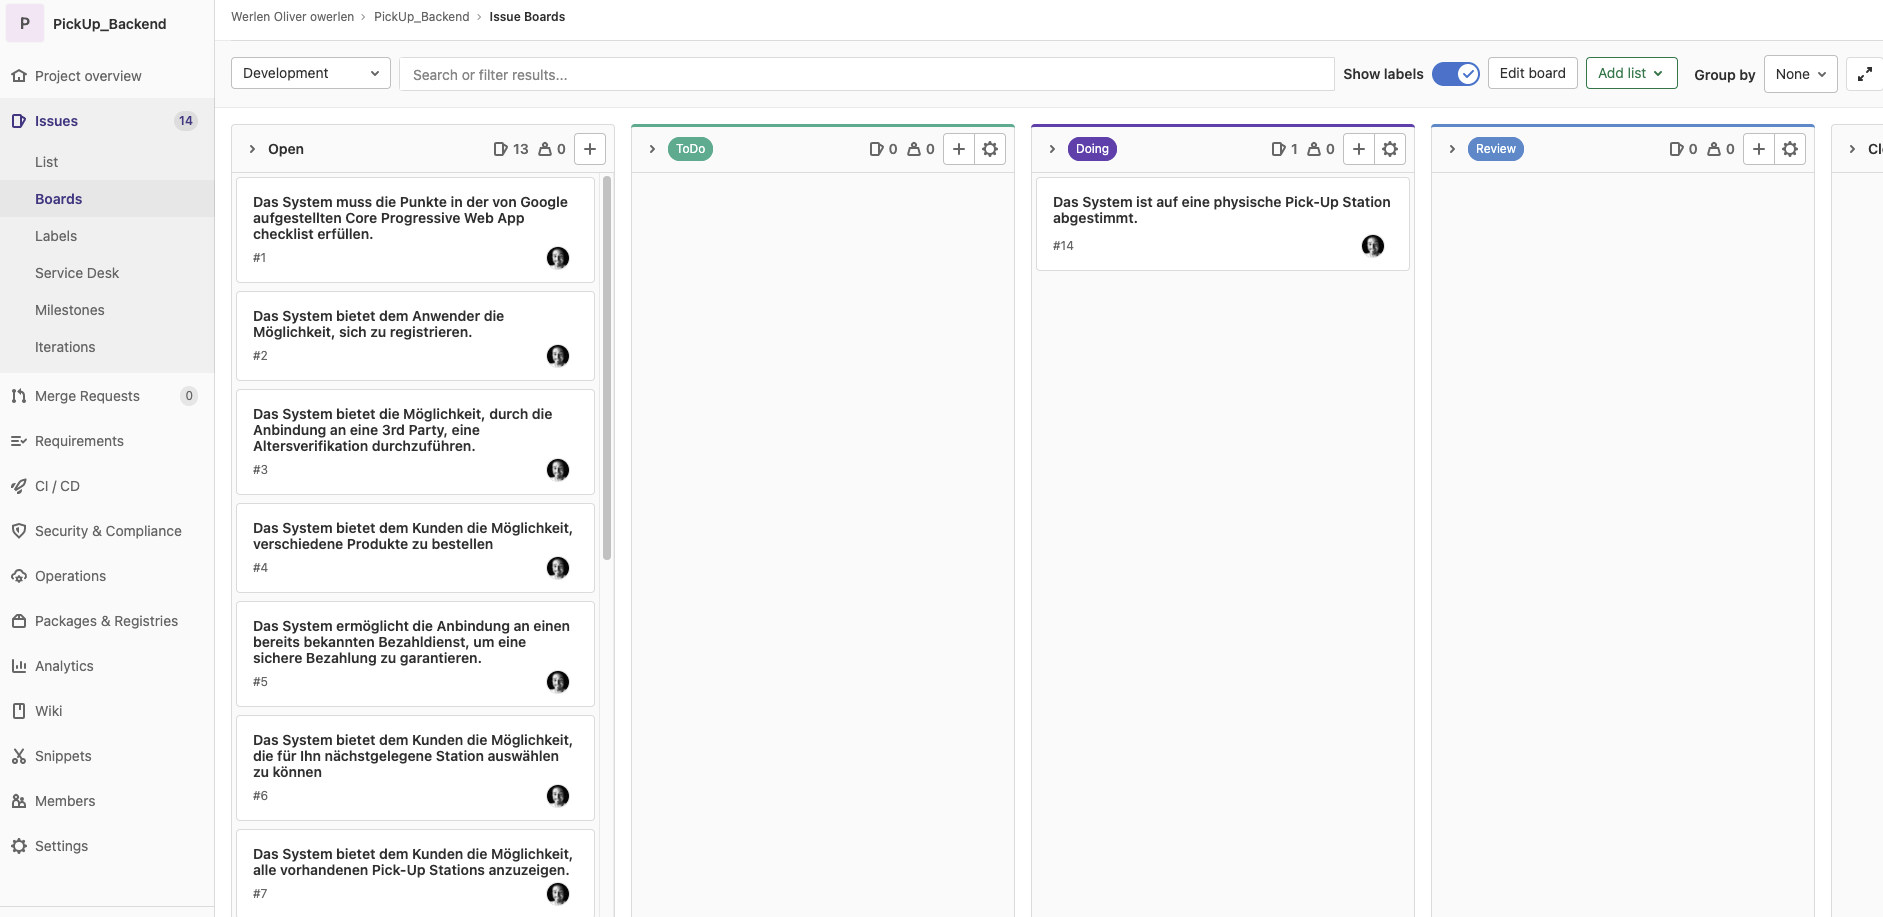
\includegraphics[width=1\textwidth]{images/boardGitlab.png}
	\caption[GitLab Board]{GitLab Board,\\ Quelle: Autor}
	\label{img: GitlLabBoard}
\end{figure}
Für die Sprint Planung werden einzelne User Stories verschoben. Beim Sprint Review werden die Stories in "reviewing" mit den definierten Akzeptanzkriterien mit den Resultaten verglichen. Basierend darauf wird entschieden, ob an der \gls{User Story} noch weiter gearbeitet werden, das heisst zurück zu "doing" oder die Story in "done" verschoben werden kann. Bei Beginn des nächsten Sprints wird das Vorgehen wiederholt. \\
Die einzelnen Items sind dabei priorisiert. Elemente mit einer hohen Einstufung werden dabei bei der Bearbeitung vorgezogen. 

\subsection{CI/CD}
\begin{figure}[H]
	\centering
	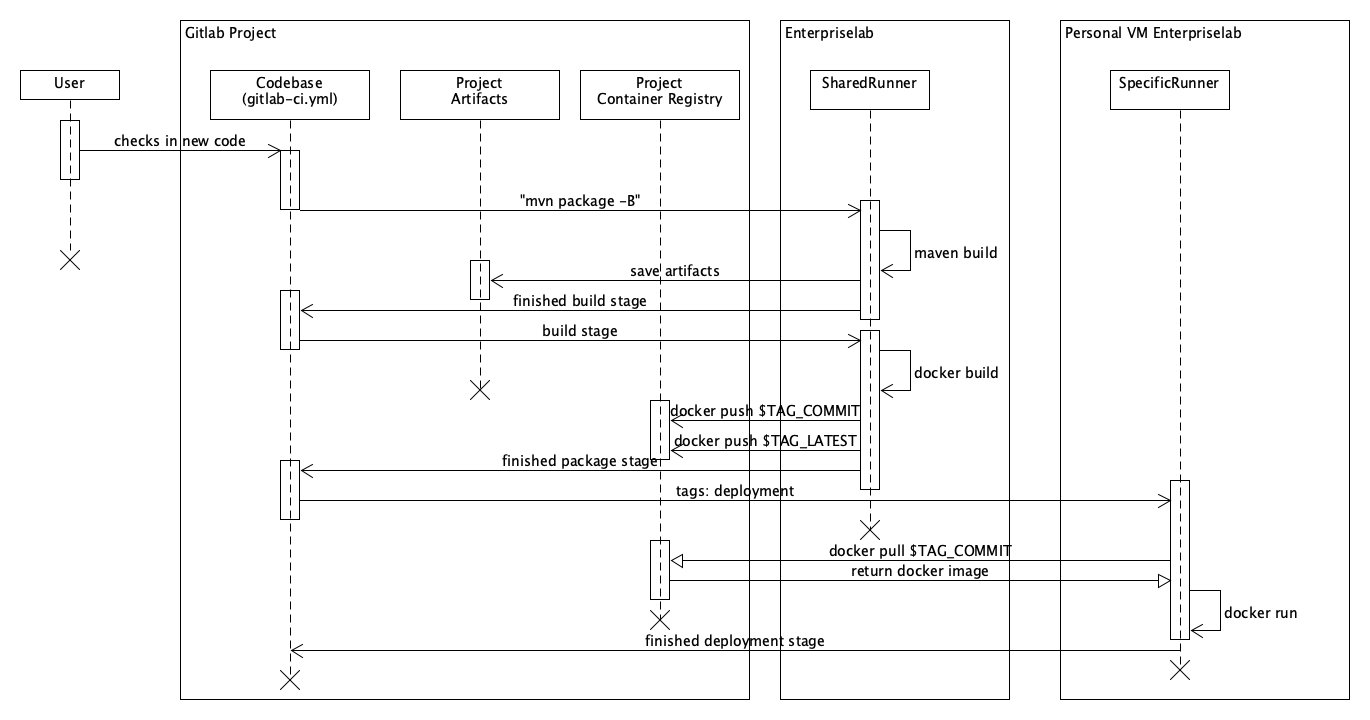
\includegraphics[width=1\textwidth]{images/sequenceCicd.png}
	\caption[Ablauf der CI/CD Pipeline]{Ablauf der CI/CD Pipeline,\\ Quelle: Autor}
	\label{img: cicdPipeline}
\end{figure}


\newpage